\documentclass{article}
\usepackage[utf8]{inputenc}
\usepackage{geometry}
 \geometry{
 a4paper,
 total={170mm,257mm},
 left=20mm,
 top=20mm,
 }
\usepackage{polski}
\usepackage{natbib}
\usepackage[capbesideposition=right]{floatrow}
\usepackage{graphicx}
\usepackage{pbox}
\usepackage{float}
\usepackage[dvipsnames]{xcolor}
\usepackage{caption}
\usepackage{wrapfig}
\usepackage{graphicx}
\usepackage{tikz}
    \usetikzlibrary{
        arrows,
        shadows,
        shapes,
        automata,
        positioning,
        arrows.meta
    }
\usepackage{pgfplots}
\usepackage{tabularx}
\usepackage{booktabs}
\usepackage{amsfonts}
\pgfplotsset{compat=1.17}

\begin{document}
\centering
\Huge{Activity diagram of a card generation}
\normalsize
\vspace{2cm}

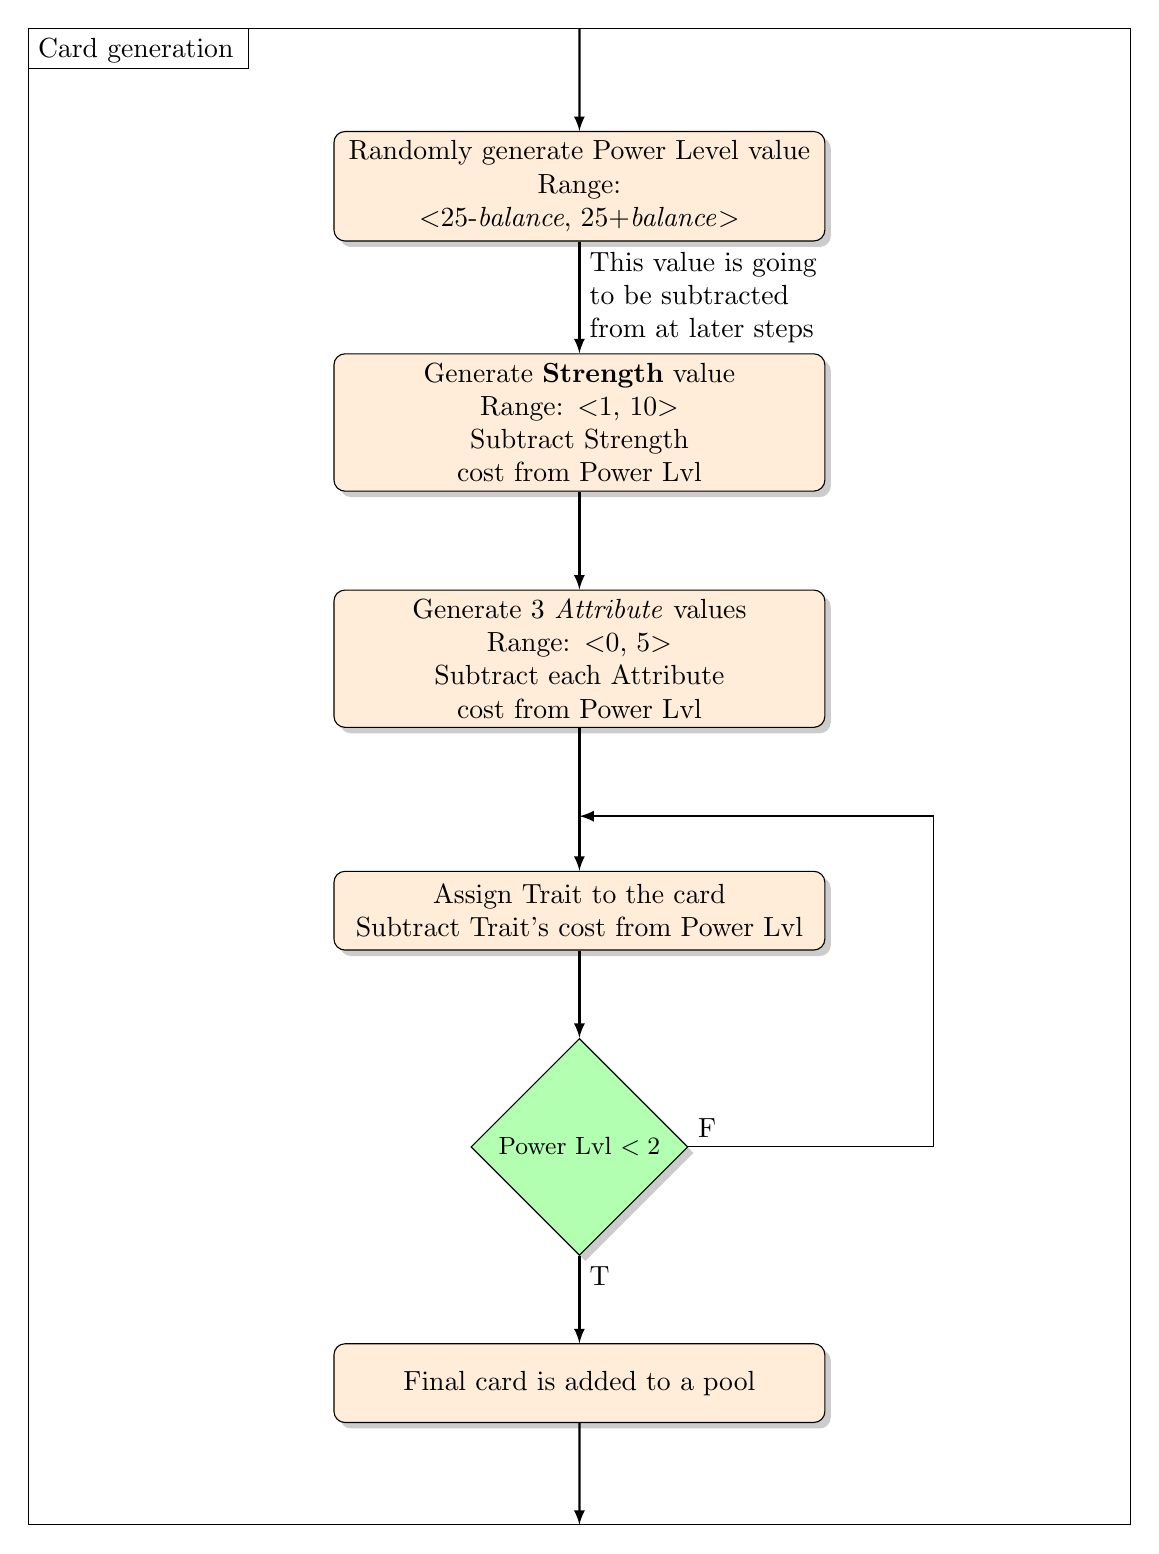
\begin{tikzpicture}
[baseshape/.style={minimum width=3.5cm, minimum height=1cm,text centered, font=\normalsize,draw=black, drop shadow=black!40},
startstop/.style={baseshape, ellipse, fill=red!30},
io/.style={baseshape, trapezium, trapezium stretches=true, 
trapezium left angle=70, trapezium right angle=110, fill=blue!30},
process/.style={baseshape, rectangle, rounded corners, text width=6cm, fill=orange!15},
decision/.style={baseshape, diamond, minimum width=1cm, fill=green!30},
arrow/.style={thick, -latex},
node distance=3cm,]
    \node (step1) [process, xshift = 3cm, yshift = -1cm] {Randomly generate Power Level value \\ Range: \\ $<$25-\textit{balance}, 25+\textit{balance}$>$};
    \node (step2) [process, below of=step1] {Generate \textbf{Strength} value \\ Range: $<$1, 10$>$ \\ Subtract Strength cost from Power Lvl};
    \node (step3) [process, below of=step2] {Generate 3 \textit{Attribute} values \\ Range: $<$0, 5$>$ \\ Subtract each Attribute  \\ cost from Power Lvl };
    \node (step4) [process, below of=step3, yshift = -0.2cm] {Assign Trait to the card \\ Subtract Trait's cost from Power Lvl};
    \node (step5)[decision, below of=step4] {\small{Power Lvl }$ < 2$};
    \node (step6) [process, below of=step5] {Final card is added to a pool};
    \draw[arrow] (3,1) -- (step1);
    \draw[arrow] (step1) -- node[at start, anchor=north west, text width = 3cm]{This value is going to be  subtracted from at later steps}(step2);
    \draw[arrow] (step2) -- (step3);
    \draw[arrow] (step3) --  coordinate(a)(step4);
    \draw[arrow] (step4) -- (step5);
    \draw (step5) -| node[at start, anchor=south west]{F}(7.5, -9);
    \draw[arrow] (7.5,-9) -- (3,-9);
    \draw[arrow] (step5) -- node[at start, anchor=north west] {T} (step6);
    \draw[arrow] (step6) -- (3,-18);
    
    \draw (-4,1) -- node[at start, anchor=north west]{Card generation}(-1.2,1) -- (-1.2, 0.5) -- (-4, 0.5) -- (-4, 1) -- (10, 1) -- (10, -18) -- (-4,-18) -- (-4, 1);
\end{tikzpicture}

\clearpage

\Huge{Example of a single card generation}
\normalsize
\vspace{2cm}

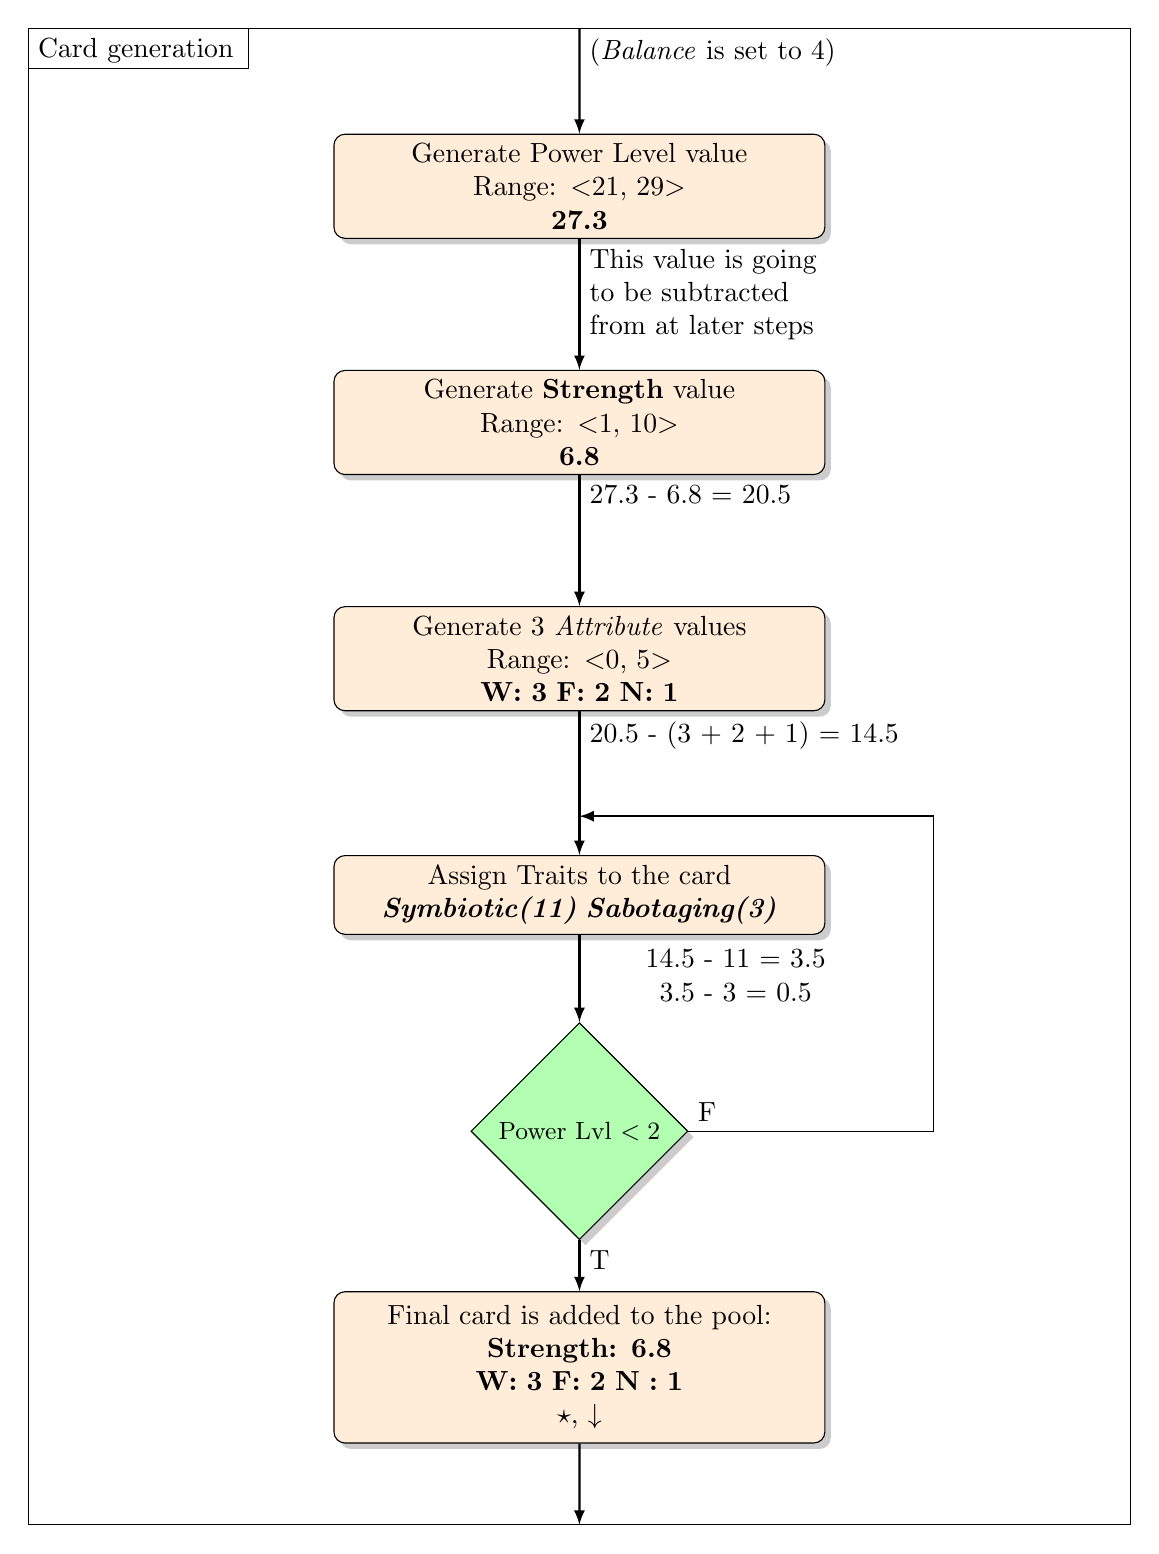
\begin{tikzpicture}
[baseshape/.style={minimum width=3.5cm, minimum height=1cm,text centered, font=\normalsize,draw=black, drop shadow=black!40},
startstop/.style={baseshape, ellipse, fill=red!30},
io/.style={baseshape, trapezium, trapezium stretches=true, 
trapezium left angle=70, trapezium right angle=110, fill=blue!30},
process/.style={baseshape, rectangle, rounded corners, text width=6cm, fill=orange!15},
decision/.style={baseshape, diamond, minimum width=1cm, fill=green!30},
arrow/.style={thick, -latex},
node distance=3cm,]
    \node (step1) [process, xshift = 3cm, yshift = -1cm] {Generate Power Level value \\ Range: $<$21, 29$>$ \\ \textbf{27.3}};
    \node (step2) [process, below of=step1] {Generate \textbf{Strength} value \\ Range: $<$1, 10$>$\\ \textbf{6.8}};
    \node (step3) [process, below of=step2] {Generate 3 \textit{Attribute} values \\ Range: $<$0, 5$>$ \\ \textbf{W: 3 F: 2 N: 1}};
    \node (step4) [process, below of=step3, label=below right:{\begin{tabular}{c}
         14.5 - 11 $=$ 3.5  \\ 3.5 - 3 $=$ 0.5
    \end{tabular} }] {Assign Traits to the card \\ \textit{\textbf{Symbiotic(11) Sabotaging(3)}}};
    \node (step5)[decision, below of=step4] {\small{Power Lvl }$ < 2$};
    \node (step6) [process, below of=step5] {
    \begin{tabular}{c}
         Final card is added to the pool:  \\
         \textbf{\textbf{Strength}: 6.8} \\
         \textbf{W: 3 F: 2 N : 1} \\
         $\star$,  $\downarrow$
    \end{tabular}};
    \draw[arrow] (3,1) -- node[at start, anchor=north west, text width = 4cm]{(\textit{Balance} is set to 4)}(step1);
    \draw[arrow] (step1) -- node[at start, anchor=north west, text width = 3cm]{This value is going to be  subtracted from at later steps}(step2);
    \draw[arrow] (step2) -- node[at start, anchor=north west]{27.3 - 6.8 = 20.5}(step3);
    \draw[arrow] (step3) --  node[at start, anchor=north west]{20.5 - (3 + 2 + 1) = 14.5}(step4);
    \draw[arrow] (step4) -- (step5);
    \draw (step5) -| node[at start, anchor=south west]{F}(7.5, -9);
    \draw[arrow] (7.5,-9) -- (3,-9);
    \draw[arrow] (step5) -- node[at start, anchor=north west] {T} (step6);
    \draw[arrow] (step6) -- (3,-18);
    
    \draw (-4,1) -- node[at start, anchor=north west]{Card generation}(-1.2,1) -- (-1.2, 0.5) -- (-4, 0.5) -- (-4, 1) -- (10, 1) -- (10, -18) -- (-4,-18) -- (-4, 1);
\end{tikzpicture}
\end{document}